\chapter{Estudo do Estado da Arte}
\label{chap:metod}
Nessa pesquisa foram abordados diversos aspectos que envolvem o desenvolvimento de um projeto de criação de um UAV do tipo quadrotor. O desenvolvimento de uma plataforma desse tipo envolve desafios estruturais, autonomia, controle, localização, planejamento de trajetória, entre outros, que necessitam de estudo prévio detalhado para ser alcançado um bom resultado com o veículo.

% %--------- NEW SECTION ----------------------
\section{Quadrotores}
% \label{sec:ui}
Quadrotores são aeronaves de asas rotativas, ou seja, são sustentadas e movimentadas por rotores. Diferente das aeronaves de asas fixas, como aviões, as aeronaves de asas rotativas não utilizam seu movimento horizontal para sustentar seu vôo. Isso faz com que esse tipo de veículo apresente um consumo energético muito alto \cite{karydis2017energetics}. Apesar disso, as aeronaves de asas rotativas possuem a habilidade de realizar pouso e decolagem vertical e também de realizar vôos estacionários ou quase estacionários.

As aeronaves de asas rotativas são classificadas como multirrotores, sendo classificadas quanto ao número de propulsores que elas possuem, podendo ser: quadrotores, hexarotores, octarotores, coaxiais ou helicópteros. Os quadrotores são veículos que apresentam alta manobrabilidade e alto payload, mas apresentam também alto gasto energético, tornando baixa o seu tempo de vôo, sendo um desafio achar baterias mais eficientes que aumentem sua autonomia. A medida que aumenta-se o número de rotores, passando de quadrotores para hexarotores e octarotores, aumenta-se também o payload, que é o quanto a aeronave consegue carregar em relação ao seu peso, e a tolerância a falha, que é a habilidade continuar realizando um vôo controlado mesmo com alguns rotores apresentando falhas de funcionamento. Entretanto, diminui-se também a manobrabilidade e aumenta-se o consumo energético.

Os movimentos do quadrotor são obtidos através da combinação das velocidades angulares dos rotores, como mostrado na Figura \ref{fig:movimentos}. Para balancear o contra-torque gerado por seus propulsores, é necessário que um par de rotores que estão em uma mesma haste esteja girando no sentido horário, enquanto o outro par de rotores esteja girando no sentido anti-horário. Para um quadrotor realizar movimentos verticais é necessário aumentar ou diminuir a velocidade dos quatro rotores simultaneamente. Para um quadrotor de translação horizontal, é necessário manter a velocidade de rotação de um par de rotores igual, enquanto a velocidade de rotação do outro par de rotores no sentido do movimento é desbalanceada, fazendo com que o quadrotor se incline, no caso de um quadrotor em configuração em "+". Para realizar o movimento de rotação em torno do eixo vertical, conhecido como movimento de guinada. é necessário que a velocidade de um par de rotores seja superior a velocidade de rotação do outro par, fazendo com que o contra-torque resultante não seja nulo. \cite{Bouabdallah2007}

\begin{figure} [h!]	
  \centering
  \caption{Movimentos do Quadrotor}
  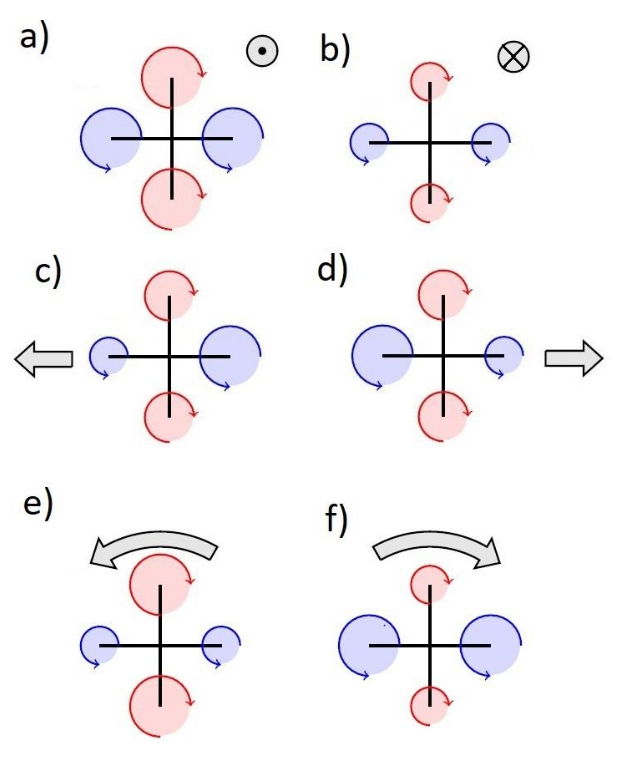
\includegraphics[width=0.6\textwidth]{Figures/Screenshot from 2021-12-14 15-46-58.png}
  \caption*{Fonte: \cite{monteiro2015modelagem}, adaptada.}
  \label{fig:movimentos}
\end{figure}

\subsection{Classificações}
Os quadrotores são classificados em categorias, possuindo cada uma delas características específicas, que podem ajudar no design do projeto e também na escolha de componentes que vão ajudar na operação da aeronave.

\subsubsection{Classificação Quanto ao Peso}
L. Brooke-Holland, Unmanned Aerial Vehicles (drones): An Introduction, House of

Em \cite{brooke2012unmanned}, Os UAVs são classificados em categorias de acordo com o quanto eles pesam. UAVs que pesam até 200 gramas (g) são classificados como nano drones, de 200 g até 2 quilogramas (kg) são classificados como micro drones, de 2 kg até 20 kg são classificados como mini drones, de 20 kg até 150 kg, como small drones, de 150 kg até 600 kg, como tactical drones e de 600 kg em diante são classificados como MALE, HALE ou Strike drones. Segundo a Agência Nacional de Aviação Civil (ANAC) \cite{ANAC2021}, os drones que pesam mais que 150 kg são classificados como Classe 1, os drones de 25 kg até 150 kg são classificados como Classe 2 e os drone de até 25 kg são classificados como Classe 3, sendo dividida esa classe em drone de até 250 g e drone de 250 g até 25 kg. Cada classificação dessa possui regulamentação específica. Quadrotores mais leves são mais ágeis por serem menores e, consequentemente, terem inércias menores. Possuindo assim maiores acelerações angulares e lineares.

\subsubsection{Classificação Quanto a Configuração}
Os quadrotores tem duas configurações possíveis em relação à disposição de seus rotores. Os rotores podem ter a a configração em forma de "+", em que a frente da aeronave fica alinhada com uma das hastes que suporta um par de rotores. Essa configuração também é conhecida como cruz. A outra configuração possível é a configuração em "x", em que a frente da aeronave fica a 45$^{\circ}$ do eixo que contém a haste da aeronave, ficando assim a frente da aeronave no meio de duas hastes, como mostrado na Figura \ref{fig:configs}, em que o eixo x está orientado positivamente para a frente da aeronave. 

\begin{figure} [h!]	
  \centering
  \caption{Configurações}
  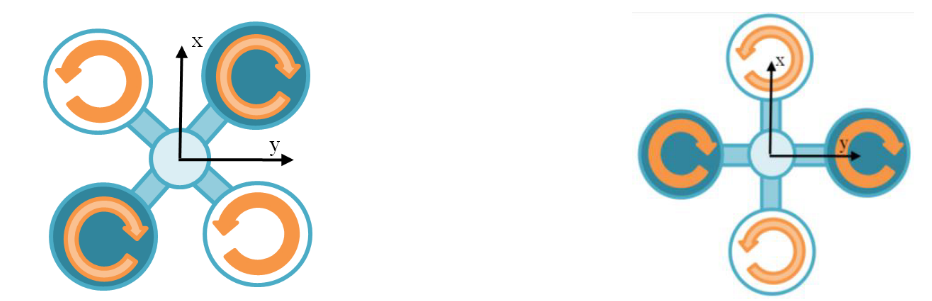
\includegraphics[width=1\textwidth]{Figures/configs.png}
  \caption*{Fonte: \cite{NorouziGhazbi2016}}
  \label{fig:configs}
\end{figure}

A configuração em "+" é mais acrobática, entretanto, como desvantagens, a haste dos rotores bloqueia o campo de visão da câmera e também apresenta um momento de guinada ao transladar, necessitando de um maior gasto energético para estabilizar a aeronave.

A configuração em "x" não apresenta esse efeito, por ter os movimentos de arfagem e rolagem desacoplados do de guinada. Apresenta menor esforço para transladar pois todos rotores agem nesses movimentos, diferente da configuração em "+", em que apenas um par de rotores é responsável pelo deslocamento enquanto o outro se mantém com velocidades constantes. É mais estável, entretanto apresenta menor manobrabilidade. \cite{NorouziGhazbi2016}

% \subsubsection{Ambiente de Operação}
% Os quadrotores podem operar em dois tipos de missões: outdoor e indoor. As missões outdoor são as missões em que os quadrotores são expostos a ambientes desconhecidos, onde existe a forte presença de pertubações, como rajadas de vento. Nesse tipo de missão, os quadrotores muitas vezes vão precisar de sensores do tipo GPS para ajudar na localização do veículo e também de um controlador adequado para lidar com a rejeição de pertubação. As missões indoor possuem menos pertubações e ambientes mias estruturados. Sendo possível fazer o mapeamento prévio do ambiente para realizar as operações 

\subsection{Principais Componentes}

Os principais componentes envolvidos no desenvolvimento de um VANT do tipo quadrotor são os rotores que serão responsáveis por toda movimentação do drone, baterias que irão garantir a energia necessária para os rotores, sensores inerciais que irão ser responsáveis pela localização do drone e microcontroladores, responsáveis pelo cálculo das ações de controle e a integração de hardware e software.

\subsubsection{Sensores Inerciais}

Os VANTs são geralmente equipados com uma IMU (Inertial Measurement Unit), que são dispositivos compostos por giroscópios, acelerômetros e magnetômetros. Os giroscópios são sensores capazes de medir a velocidade angular do veículo nos três eixos, os acelerômetros são responsáveis por calcular as acelerações lineares nos três eixos e o magnetômetro mede campos magnéticos também nos três eixos. Devido ao forte campo magnético existente no planeta Terra, é possível obter a orientação do robô através da obtenção da magnitude do campo magnético atuando no eixos da aeronave. Através da fusão sensorial é possível obter a atitude do robô e realizar odometria. Muita vezes também são utilizados sensores do tipo barômetro, que são sensores capazes de medir a pressão atmosférica. Como a pressão atmosférica varia com a altitude, é possível mensurar a altura da aeronave em relação ao nível do mar com a utilização desse sensor.

\subsubsection{Motores}

% Falar sobre hélices?

Como a alimentação do quadrotor ser a base de baterias de corrente contínua é adequado que sejam utilizados motores que utilizem esse tipo de alimentação. Os motores DC são máquinas elétricas de corrente contínua (CC) que são constituídos por uma armadura ou rotor, que é a parte giratória montada sobre o eixo da máquina, um estator de material ferromagnético envolvido pelo enrolamento de campo, um comutador com função de manter o torque gerado em um determinado sentido e de escovas, que são conectores fixos que permitem o deslizamento do comutador no eixo da armadura. Os motores DC possuem uma grande variabilidade de velocidade de operação, podendo operar acima e abaixo do valor nominal, possuem alta aceleração, podendo variar de velocidade rapidamente, inclusive mantendo o torque constante e não necessitam de conversores complexos. Como desvantagens, eles necessitam de manutenção constante para a troca de escovas, são mais caros e maiores do que motores CA com mesma potência e também possuem centelhamento.

O motor brushless DC (BLDC) é um motor de corrente contínua síncrono que é alimentado por corrente contínua (CC) e não possui escovas de contato elétrico. Ele é composto por imãs permanentes, chamados de magnetos, que podem ser localizados no estator externo ou no centro no estator interno. A vantagem desse tipo de motor é que eles são altamente eficientes, pois possuem menos perdas por atrito, resultando em torques maiores. Essa eficiência é de grande valia para os quadrotores, pois um grande desafio associado a operação com esse tipo de veículo é a autonomia. A redução do atrito também faz com que a vida útil desse tipo de motor seja maior e que seja necessário ter menos manutenções, por não necessitar trocar as escovas. Sendo esse tipo de motor uma ótima opção de escolha para o desenvolvimento de um drone.

\subsubsection{Baterias}

Um grande desafio a ser enfrentado no trabalho com veículos aéreos de asas rotativas é a autonomia. Graças ao grande gasto energético que essas aeronaves possuem para se sustentar no ar, o tempo de vôo desses veículos acaba se tornando baixo.   

As baterias mais amplamente utilizadas para UAVs são baterias polímero de lítio (LiPo). Esse tipo de bateria tem uma das melhores relações entre capacidade e peso, o que é de vital importância para esse tipo de veículo, já que o peso das baterias pode representar até 50\% do peso da aeronave, como mostrado em \cite{Mulgaonkar2014}. As baterias LiPo possuem uma capacidade regular e um bom ciclo de vida. Em \cite{Abdilla2015b}, é feito um estudo do consumo de energia de multirrotores e uma modelagem para estimação da autonomia do veículo operando com baterias LiPo.  

% recarga wireless?

\subsubsection{Microcontrolador}

O microcontrolador é responsável por realizar a comunicação entre componentes e funcionalidades e a implementação do controlador que irá atuar nos propulsores. Existem diversos modelos no mercado, com diferentes frequências de operação ou clock, memória flash, RAM, EEPROM e tensão de alimentação. O clock determina quantas operações o microprocessador consegue fazer por unidade de tempo, quanto maior essa velocidade, menor é o tempo entre ações de controle, tornando o controle mais preciso. Entre as plataformas mais utilizadas estão o Arduino, a Raspberry, ARM, PIC, ESP32 e Teensy. A plataforma Arduino é baseada em chips ATmega, chegando a frequência máxima de 84 Mhz em seu modelo Arduino DUE, com SRAM de 96 kB e memória flash de 512 kB. A plataforma Raspberry Pi utiliza chips ARM, sendo seu modelo raspberry Pi 4 utilizando 4 núcleos ARM com 1.5 Ghz de clock. A plataforma Teensy é baseado em chips ARM, seu modelo teensy 4.0 apresenta um chip ARM Cortex-M7 de 600mHz. Como mostrado em um benchmark que são medidos o número de operações por segundo dos microcontroladores fazendo tarefas comuns, mostrado na Figura x, mas que não inclui a Raspberry Pi 4, o Teensy 4.0 aparece como muito superior a todas outras opções.

\begin{figure} [h!]	
  \centering
  \caption{Benchmark dos Microcontroladores}
  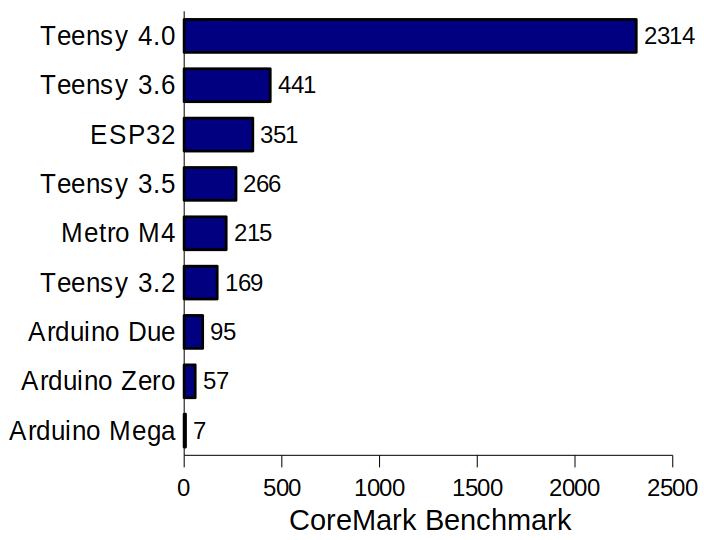
\includegraphics[width=0.7\textwidth,trim={0 0.8cm 0 0},clip]{bench.png}
  \caption*{Fonte: \cite{benchmark}}
  \label{fig:BILI}
\end{figure}

%-----------------------------------------------------
\section{Funcionalidades}
% \label{sec:ui}

As principais funcionalidades que compõe uma plataforma do tipo quadrotor são controle, localização e planejamento de trajetória. A modelagem é abordada também na discussão que segue.

\subsection{Modelagem}
A modelagem de um quadrotor é uma das etapas mais importantes no desenvolvimento de um projeto envolvendo esse tipo de veículo. Por ser uma plataforma instável, se torna inviável realizar técnicas de identificação em malha aberta. Sendo assim, é necessário obter o modelo dinâmico da aeronave através de técnicas de modelagem.

A modelagem da aeronave pode ser obtida através das equações de Newton-Euler ou através do formalismo de Euler-Lagrange \cite{castillo2005modelling} . Através dessa modelagem é possível obter o modelo de alto nível, onde os torques e forças são entradas e as saídas são posições angulares e lineares. 

\subsection{Controle}
Os quadrotores são veículos subatuados, ou seja, possuem mais graus de liberdade do que atuadores, são naturalmente instáveis e apresentam comportamento não-linear. Devido a esses fatores, esse tipo de veículo necessita de uma estrutura de controle adequada bem ajustada para que seja possível a estabilização e o seguimento de referência.

Os controladores que atuam no quadrotor geralmente são utilizados em cascata \cite{Nonami2010a}, de forma que existe um controle de baixo nível para garantir uma velocidade de rotação desejada nos rotores, um controlador em um nível mais alto para controlar a altitude e as velocidade angulares de rolagem, arfagem e guinada e por último um controlador no nível mais alto controlando posições lineares no espaço tridimensional \cite{Kendoul2007}, formando assim uma estrutura de controle hierárquica.

Os controlador mais comumente usado em baixo nível para controlar a velocidade de de rotação dos propulsores é o controlador Proporcional Integral Derivativo (PID) já que os rotores são sistemas SISO (single-input single-output) que podem ser representado por dinâmicas de primeira ordem.

Os controladores que controlam atitude, altitude e posições lineares no quadrotor podem ser controladores lineares ou não-lineares. Para serem utilizados controladores lineares é necessário realizar uma linearização em um ponto de operação no modelo matemático do quadrotor, considerando pequenas variações de ângulo.

Os controladores lineares que são mais amplamente utilizados são os controladores PID, LQR e H$\infty$. Como alguns parâmetros do quadrotor podem apresentar incertezas ou até mesmo variar durante a operação, sendo possível adicionar robustez a esses controladores, podendo ajudar também na rejeição de perturbação. 

O controlador PID é um controlador prático e de fácil implementação que pode ser usado sem o conhecimento da dinâmica do sistema ajustando os parâmetros empiricamente. A técnica foi uma das primeiras a ser utilizada e é constantemente utilizada como parâmetro de comparação para outras técnicas. Foi implementado com sucesso em trabalho como \cite{bouabdallah2004design,Hoffmann2007}.

O Regulador Quadrático Linear (LQR) é um controlador de realimentação de estado que minimiza uma função custo que pondera o sinal de controle e o erro do segmento de referência. Foi implementado com sucesso em \cite{bouabdallah2004design,waslander2005multi}.

O controlador H$\infty$ é um controlador por realimentação de estado que minimiza a norma H$\infty$ através da solução de desigualdades matriciais lineares. O quesito de robustez pode ser facilmente adicionado nessa técnica solucionando o problema de otimização para um politopo convexo. O controlador se mostra eficiente em lidar com pertubações. Em \cite{raffo2008backstepping}, é utilizado um controlador H$\infty$ não linear robusto para estabilizar a orientação da aeronave enquanto a técnica de Backstepping é utilizada para controlar as posições se mostrando eficiente para controlar o sistema com a presença de perturbações e incertezas paramétricas. A ação integral também pode ser utilizada para aprimorar os resultados, como mostrado em \cite{Raffo2010}.

Os controladores não-lineares mais amplamente utilizados são backstepping, o sliding mode control (SMC) e o controlador Fuzzy.

A técnica de sliding mode control (SMC) é um método de controle não-linear baseado do critério de estabilidade de lyapunov, que atinge seu objetivo através da definição de uma superfície de deslizamento onde estarão as trajetórias do sistema que são atingidas através de funções de chaveamento. O SMC é uma técnica que une robustez com velocidade de convergência, o que permite a aeronave realizar missões de difíceis trajetórias, lidar com grandes variações de parâmetros e pertubações. A técnica SMC também permite construir um observador de estados, para aplicações em que a medição de determinados pode se encontrar ausente ou falhar por alguns instantes. Em \cite{Zhao2018a} foi utilizada a um SMC adaptativo utilizando a técnica de backstepping em um quadrotor e comparados os resultados com o PID e com o SMC padrão em ambiente de simulação, mostrando que o SMC adaptativo apresenta melhores resultados.

A técnica Backstepping é uma técnica de controle não linear recursiva baseada também no critério de Lyapunov, que obtêm um controlador que estabiliza a aeronave formalmente. Essa é uma técnica que se encaixa bem em uma arquitetura de controle em cascata cumprindo a função de controlador de atitude. A técnica se mostra eficiente para lidar com o controle da orientação da aeronave na presença de fortes pertubações. Em \cite{bouabdallah2005backstepping} é feita uma comparação entre a técnica backstepping e a técnica SMC. Em \cite{madani2006backstepping} a técnica é utilizada para estabilizar todo o sistema.

O controlador Fuzzy é feito de tal forma que entradas e saídas são mapeadas através da definição de funções de pertencimento. Em \cite{santos2010intelligent}, é aplicado um controlador Fuzzy em um quadrotor para controlar a orientação da aeronave e a altitude, enquanto as entradas era a potência designada para cada motor. A técnica Fuzzy pode ser combinada com outras técnicas de controle também. Em \cite{nicol2008robust} é utilizada uma técnica chamada Cerebellar Model Articulation Controller  (CMAC) que garante um aprendizado e adaptação rápida. O CMAC associa rede neural, com técnica fuzzy e controle adaptativo. A técnica se mostrou ser computacionalmente eficiente, mas sendo necessário ajustes para adicionar robustez. Em \cite{gautam2013control} é utilizado um self-tunning PID através de algoritmo Fuzzy. Foram obtidos resultados melhores do que um controlador PID segundo o critério de integral do erro quadrático.

\subsection{Localização}
A localização do quadrotor pode ser auxiliada por uso de diversos sensores como LiDAR, GPS, IMU, câmeras monoculares, sensores ultrassônicos e lasers.

A IMU pode ser utilizada para a funcionalidade de localização através da odometria, podendo contar com giroscópio, acelerômetro, magnetômetro e até mesmo barômetro. Em \cite{loianno2016estimation}, a localização de um quadrotor é realizada utilizando a fusão sensorial de uma câmera monocular com uma IMU.

Em \cite{tomic2012toward}, é feito a odometria da aeronave através da fusão sensorial feita por Filtro Estendido de Kalman de sensores laser com câmera estéreo, em aplicações de busca e resgate em ambiente urbano.

Os sensores que são mais amplamente utilizados atualmente são os sensores baseados em visão. É possível obter bons resultados apenas utilizando câmeras monoculares, como mostrado em \cite{mur2015orb} utilizando o pacote ORB SLAM.

Os sensores GPS são amplamente utilizados para missões outdoor e os sensores ultrassônicos e baseados em laser são utilizados para auxiliar na medição da altitude.

Pode-se realizar a fusão sensorial de diversos sensores para se obter uma boa estimativa da localização da aeronave. A técnica mais amplamente utilizada é a de filtragem, como a do filtro estendido de kalman (EKF), porém ela sofre com o drift, que é um deslocamento não considerado pela medição. Outra opção são frameworks de otimização não-linear, que apresentam resultados mais consistentes, porém apresentam custos computacionais superiores.

\subsection{Planejamento de Trajetória}
O planejamento de trajetória é fundamental para que o quadrotor se torne uma plataforma completamente autônoma. Através dessa funcionalidade o veículo pode calcular uma rota para se deslocar da sua posição atual até uma posição final sem a interferência humana, sendo de extrema importância para o objetivo final do projeto que é tornar o drone capaz de realizar um pouso autônomo em uma plataforma móvel.

% Diversas técnicas de planejamento de trajetória tem sido usados para lidar com o problema Belief Roadmap (onde eu vi?), A*, algoritmo? genéticos, e algoritmos com inteligência artificial

Em \cite{Roberge2013b} foi feito um estudo de comparação entre o planejamento de trajetória através do algoritmo genético (GA) e da otimização por enxame de partículas (PSO) em simulação. Ambas as técnicas apresentaram boas soluções em tempos computacionais relativamente curtos . Como conclusão foi observado que com significância estatística o GA apresenta melhores trajetórias ao PSO. Para comparar os resultados foi realizar o t-teste sobre o a função custo.

Em \cite{chen2016uav} é feito o planejamento de trajetória através da técnica Artificial Potential Field (APF), que é vantajosa por ser implementada através de um algoritmo de estrutura simples, com uma descrição matemática consistente e conveniente para controle em tempo real, além de possuir uma grande portabilidade, podendo solucionar o problema de desvio de obstáculos mudando a fonte do campo potencial artificial. A técnica também pode ser utilizada para o planejamento de trajetória de vôo em formações de múltiplos UAVs. Apesar das diversas vantagens, o APF na configuração padrão não resulta na trajetória ótima, sendo possível ser combinado com outras técnicas como o algoritmo genético ou algoritmos evolucionários para melhorar seus resultados. O APF é baseado na ideia de que o destino funciona como um campo potencial atrativo para o UAV, enquanto os obstáculos funcionam como campos potenciais repulsivos. Nessa pesquisa, o APF é reconstruído sobre a otimização com restrições introduzida com a força de controle adicional.

Em \cite{chen2016modified} , é utilizado um algoritmo de otimização derivado do Central Force Optimization (CFO), chamado de Modified Central Force Optimization. O CFO é um algoritmo de otimização de partícula inteligente baseado na lei da gravidade, onde cada solução é uma partícula. As partículas se atraem com a força gravitacional virtual. As massas dessas partículas são dependentes da função custo de cada solução. Na metáfora do CFO, quando uma massa está sobre forte influência de uma massa, ela fica presa em seu campo gravitacional, o que é análogo a localizar um valor máximo para uma função objetivo.
No MCFO são adicionados conceitos da otimização por Enxame de partículas (PSO) além do operador de mutação do algoritmo genético (GA) para melhorar os resultados do CFO. Os resultados da pesquisa mostraram resultados em simulação superiores aos das técnicas com o algoritmo CFO, GA, PSO e de bucas aleatórias.

Em \cite{Mueller2015a}, é apresentado um método computacional mente eficiente que calcula trajetórias com funções de posição polinomiais três vezes diferenciáveis, considerando as restrições de velocidade e aceleração do veículo. O algoritmo foi testado com a captura de uma bola arremessada.
 
% \begin{itemize}
%     \item Artificial potential field
%     \item probabilistic roadmap
%     \item belief roadmap
%     \item potential fields (PF)
%     \item Heuristic search algorithms
%     \item Optimization methods
%     \item planning under uncertainties
%     \item reactive and bio-inspired obstacle avoidance methods
% \end{itemize}

%-----------------------------------------------------
\section{Revisão Bibliográfica}

Os resultados obtidos através do método BILI apresentam a rede de cocitação e os principais autores envolvidos nas pesquisas desenvolvidas no assunto abordado.

\subsection{Rede de Cocitação}

A rede de cocitação obtida mostram uma coesão. As linhas mais fortes indicam uma proximidade maior entre as pesquisas ligadas. 
\clearpage
\begin{figure} [h!]	
    \centering
    \caption{Rede de Cocitação}
    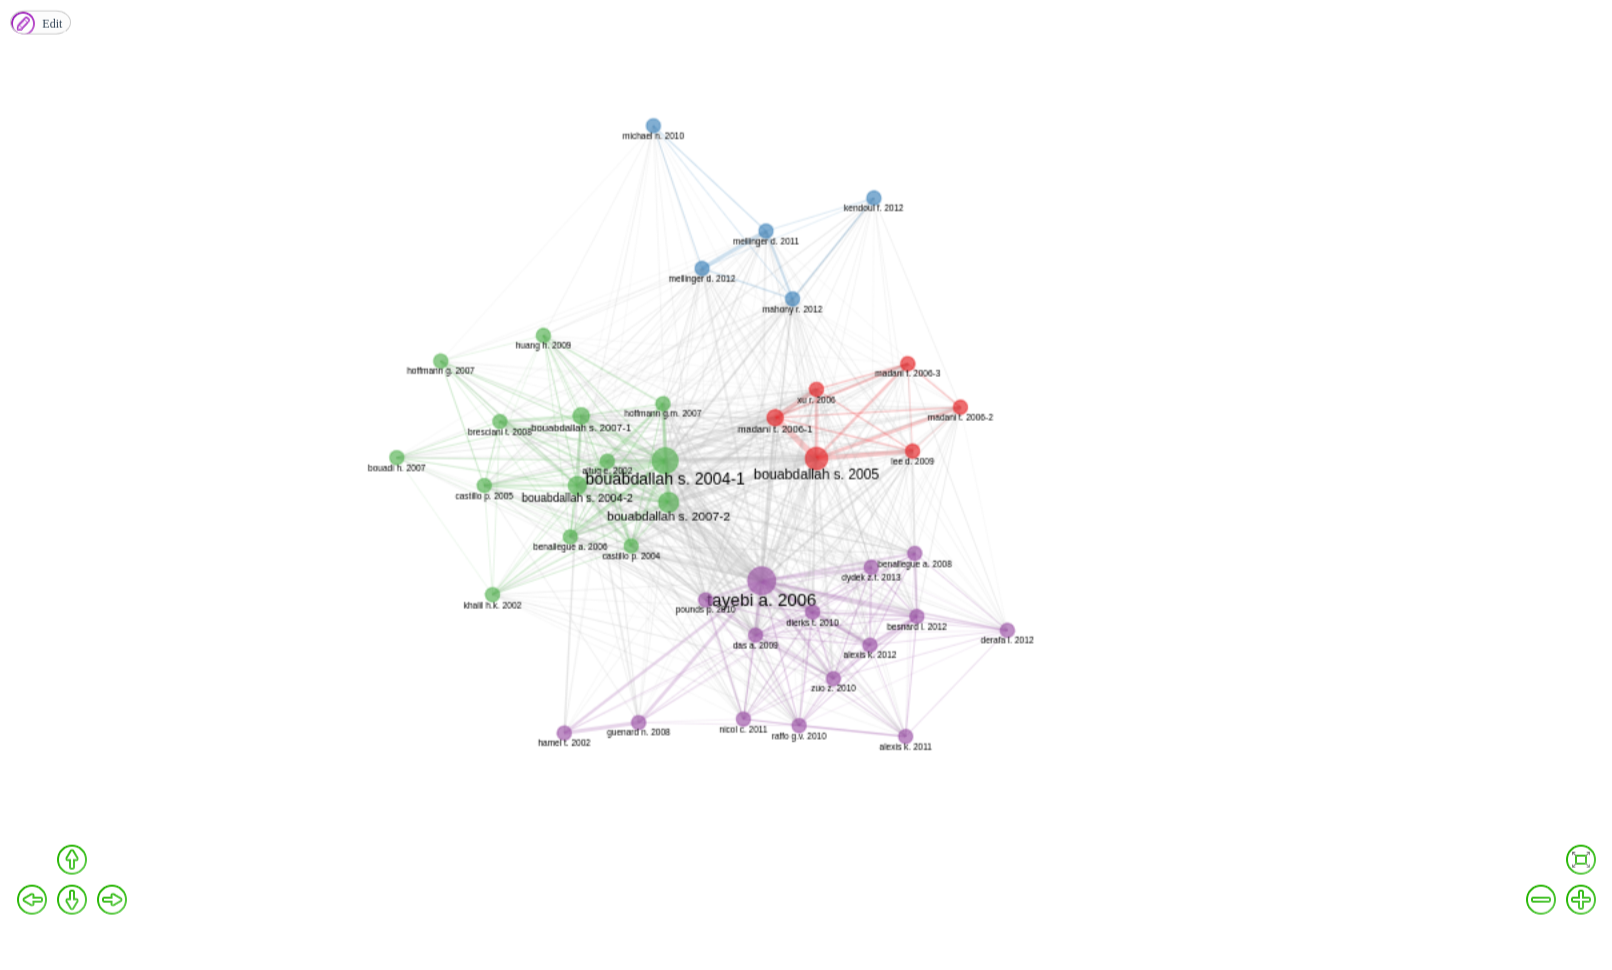
\includegraphics[width=1\textwidth,trim={3cm 6cm 3cm 
    4cm},clip,height=9cm]{Figures/network.png}
    \caption*{Fonte: Autoria própria.}
    \label{fig:cocitacao}
  \end{figure}

\subsection{Principais Autores}

Os principais autores envolvidos nas pesquisas com tema quadrotor são Kumar V., Siegwart R, Mellinger D., Bouabdallah S, como mostrado na Figura \ref{fig:autores}. e Mahony R. Bouabdalah junto com Siegwart foram um dos percursores no desenvolvimento de pesquisas sobre o design de quadrotores e controladores. Mellinger traz pesquisas na área de exploração e de planejamento de trajetória. Mahony traz pesquisas na área de pouso autônomo e Kumar diversas pesquisas com técnicas diferentes de planejamento de trajetória.

\clearpage
\begin{figure} [h]	
    \centering
    \caption{Gráfico de Total Citation}
    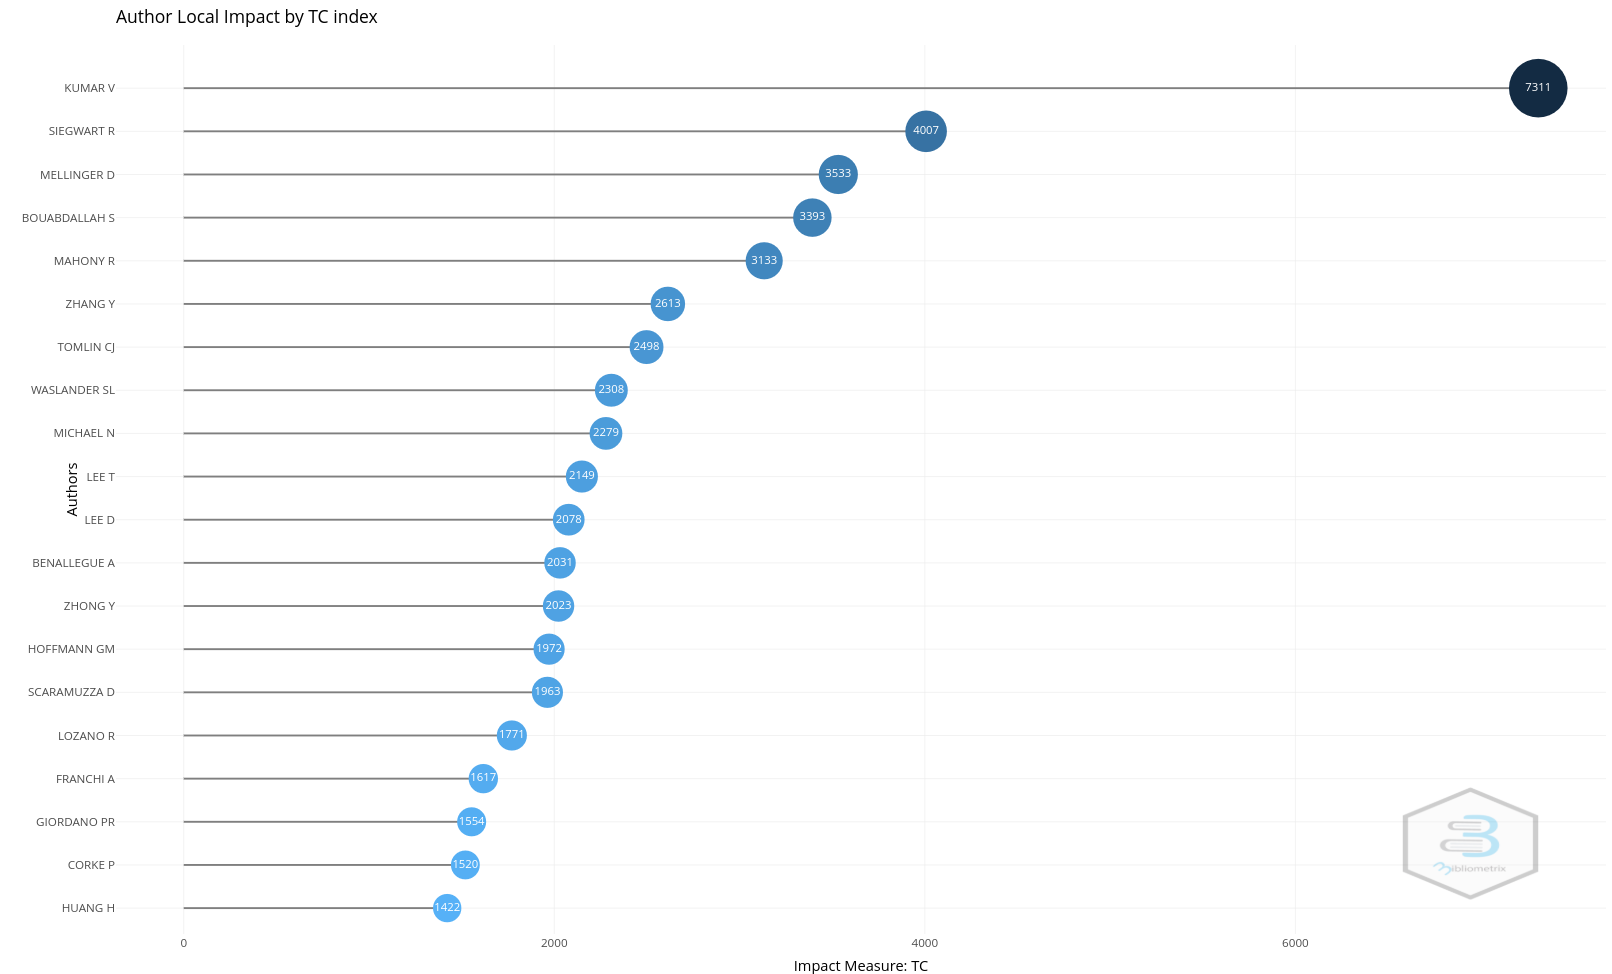
\includegraphics[width=1\textwidth,trim={0 0.8cm 0 
    1cm},clip]{Figures/newplot.png}
    \caption*{Fonte: Autoria própria.}
    \label{fig:autores}
\end{figure}

\section{Mapa Conceitual}

Foi desenvolvido um mapa conceitual para permitir uma representação visual que ajudasse a compreender os conceitos presentes nesse estudo e a relação entre eles. O mapa conceitual desenvolvido se encontra na sessão de apêndice, na Figura \ref{fig:mapac}.


%-----------------------------------------------------
% \section{Mapa Conceitual}
% % \label{sec:ui}